\documentclass{article}
\usepackage{tikz}
\begin{document}
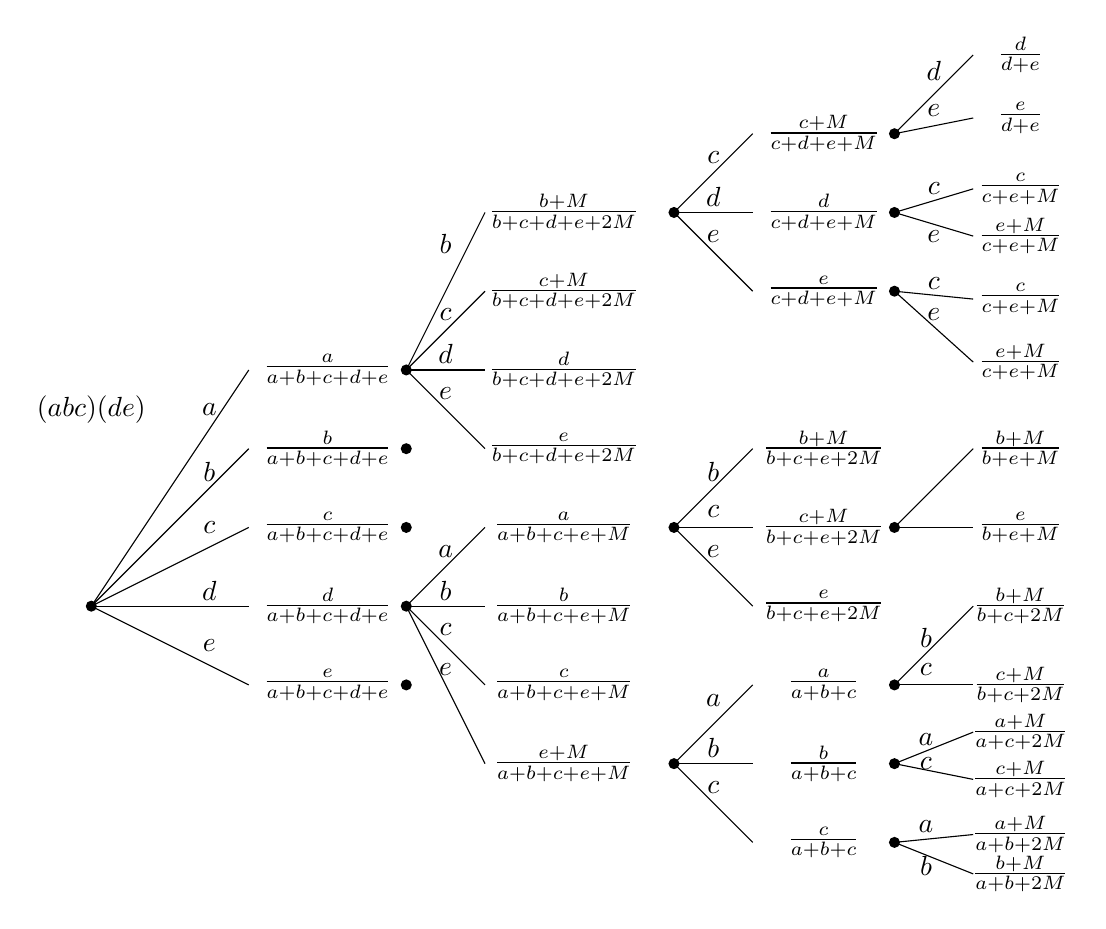
\begin{tikzpicture}
\fill (0,0) circle[radius=2pt]; % root; paths abcde
\draw (0,0) -- (2,3); 
\draw (0,0) -- (2,2);
\draw (0,0) -- (2,1);
\draw (0,0) -- (2,0);
\draw (0,0) -- (2,-1);
\node at (0,2.5) (eq1) {$(abc)(de)$};

\node at (1.5,2.5) {$a$};
\node at (1.5,1.7) {$b$};
\node at (1.5,1.0) {$c$};
\node at (1.5,0.2) {$d$};
\node at (1.5,-0.5) {$e$};

\node at (3, 3)  {$\frac{a}{a+b+c+d+e}$};
\node at (3, 2)  {$\frac{b}{a+b+c+d+e}$};
\node at (3, 1)  {$\frac{c}{a+b+c+d+e}$};
\node at (3, 0)  {$\frac{d}{a+b+c+d+e}$};
\node at (3,-1)  {$\frac{e}{a+b+c+d+e}$};

\fill  (4, 3) circle[radius=2pt];  % a finishes; paths bcde
\fill  (4, 2) circle[radius=2pt];  % terminal node
\fill  (4, 1) circle[radius=2pt];  % terminal node
\fill  (4, 0) circle[radius=2pt];  % d finishes; paths abce
\fill  (4,-1) circle[radius=2pt];  % terminal node

\draw (4,3) -- (5,5); 
\draw (4,3) -- (5,4); 
\draw (4,3) -- (5,3); 
\draw (4,3) -- (5,2); 

\node at (4.5,4.6) {$b$};
\node at (4.5,3.7) {$c$};
\node at (4.5,3.2) {$d$};
\node at (4.5,2.7) {$e$};

\node at (6, 5)  {$\frac{b+M}{b+c+d+e+2M}$};
\node at (6, 4)  {$\frac{c+M}{b+c+d+e+2M}$};
\node at (6, 3)  {$\frac{d}{b+c+d+e+2M}$};
\node at (6, 2)  {$\frac{e}{b+c+d+e+2M}$};

\fill (7.4, 5) circle[radius=2pt];  % ab finishes; pahts cde
\draw (7.4,5) -- (8.4,6);
\draw (7.4,5) -- (8.4,5);
\draw (7.4,5) -- (8.4,4);


\node at (7.9,5.7) {$c$};
\node at (7.9,5.2) {$d$};
\node at (7.9,4.7) {$e$};

\node at (9.3, 6) {$\frac{c+M}{c+d+e+M}$};
\node at (9.3, 5) {$\frac{d}{c+d+e+M}$};
\node at (9.3, 4) {$\frac{e}{c+d+e+M}$};

\fill (10.2, 6) circle[radius=2pt];  % abc finishes; paths de
\draw (10.2, 6) -- (11.2,7);
\node at (10.7,6.8) {$d$};

\node at (11.8, 7) {$\frac{d}{d+e}$};

\draw (10.2, 6) -- (11.2,6.2);
\node at (11.8, 6.2) {$\frac{e}{d+e}$};
\node at (10.7,6.3) {$e$};

\fill (10.2, 5) circle[radius=2pt];
\draw (10.2, 5) -- (11.2,5.3);
\node at (11.8, 5.3) {$\frac{c}{c+e+M}$};
\node at (10.7,5.3) {$c$};

\draw (10.2, 5) -- (11.2,4.7);
\node at (11.8, 4.7) {$\frac{e+M}{c+e+M}$};
\node at (10.7,4.7) {$e$};

\fill (10.2, 4) circle[radius=2pt];
\draw (10.2, 4) -- (11.2,3.9);
\node at (11.8, 3.9) {$\frac{c}{c+e+M}$};
\node at (10.7,4.1) {$c$};

\draw (10.2, 4) -- (11.2,3.1);
\node at (11.8, 3.1) {$\frac{e+M}{c+e+M}$};
\node at (10.7,3.7) {$e$};

\draw (4, 0) -- (5,1);
\node at (6, 1)  {$\frac{a}{a+b+c+e+M}$};

\draw (4, 0) -- (5,0);
\node at (6, 0)  {$\frac{b}{a+b+c+e+M}$};

\draw (4, 0) -- (5,-1);
\node at (6, -1)  {$\frac{c}{a+b+c+e+M}$}; 

\draw (4, 0) -- (5,-2);
\node at (6, -2)  {$\frac{e+M}{a+b+c+e+M}$};

\node at (4.5,0.7) {$a$};
\node at (4.5,0.2) {$b$};
\node at (4.5,-0.3) {$c$};
\node at (4.5,-0.8) {$e$};


\fill (7.4, -2) circle[radius=2pt];  % de finishes; paths abc
\draw (7.4, -2) -- (8.4,-1);
\draw (7.4, -2) -- (8.4,-2);
\draw (7.4, -2) -- (8.4,-3);

\node at (7.9,-1.2) {$a$};
\node at (7.9,-1.8) {$b$};
\node at (7.9,-2.3) {$c$};

\node at (9.3, -1) {$\frac{a}{a+b+c}$};
\node at (9.3, -2) {$\frac{b}{a+b+c}$};
\node at (9.3, -3) {$\frac{c}{a+b+c}$};

\fill (10.2, -1) circle[radius=2pt];  % dea finishes; paths bc
\fill (10.2, -2) circle[radius=2pt];  % deb finishes; paths ac
\fill (10.2, -3) circle[radius=2pt];  % dec finishes; paths ab

\draw (10.2, -1) -- (11.2,-0);
\node at (10.6,-0.4) {$b$};
\node at (10.6,-0.8) {$c$};


\node at (11.8, 0) {$\frac{b+M}{b+c+2M}$};
\draw (10.2, -1) -- (11.2,-1);

\node at (11.8, -1) {$\frac{c+M}{b+c+2M}$};


\draw (10.2, -2) -- (11.2,-1.6);
\node at (11.8, -1.6) {$\frac{a+M}{a+c+2M}$};

\node at (10.6,-1.7) {$a$};
\node at (10.6,-2) {$c$};

\draw (10.2, -2) -- (11.2,-2.2);
\node at (11.8, -2.2) {$\frac{c+M}{a+c+2M}$};

\draw (10.2, -3) -- (11.2,-2.9);
\node at (11.8, -2.9) {$\frac{a+M}{a+b+2M}$};

\draw (10.2, -3) -- (11.2,-3.4);
\node at (11.8, -3.4) {$\frac{b+M}{a+b+2M}$};

\node at (10.6,-2.8) {$a$};
\node at (10.6,-3.3) {$b$};

\fill (7.4, 1) circle[radius=2pt];  % da finishes; paths bce

\draw (7.4, 1) -- (8.4,2);
\draw (7.4, 1) -- (8.4,1);
\draw (7.4, 1) -- (8.4,0);

\node at (7.9,1.7) {$b$};
\node at (7.9,1.2) {$c$};
\node at (7.9,0.7) {$e$};

\node at (9.3, 2) {$\frac{b+M}{b+c+e+2M}$};
\node at (9.3, 1) {$\frac{c+M}{b+c+e+2M}$};
\node at (9.3, 0) {$\frac{e}{b+c+e+2M}$};


\fill (10.2, 1) circle[radius=2pt];  % da finishes; paths bce
\draw (10.2, 1) -- (11.2,2);
\node at (11.8, 2) {$\frac{b+M}{b+e+M}$};
\draw (10.2, 1) -- (11.2,1);
\node at (11.8, 1) {$\frac{e}{b+e+M}$};


\end{tikzpicture}
\end{document}


